\section{Boomerang Properties} \label{sec:properties}
In this section we elaborate on the anonymity and performance goals of Boomerang. We first discuss the anonymity properties that are provided by Boomerang, and then discuss system-level properties such as fault tolerance and performance.

\subsection{Anonymity Properties}
Inspired by Tarzan \cite{tarzan}, we present a simplified analysis of the anonymity properties of Boomerang with respect to static and adaptive adversaries. In particular, we strive to show that senders achieve anonymity against a minority of colluding nodes. Before proving any claims, we present the main sources of information exposure in Table \ref{tab:anonymity-properties}; a positive entry indicates that an attacker will be able to uncover the source of information, whereas a negative entry indicates that such exposure is not feasible given the Boomerang design.

\begin{table*}[t]
\begin{center}
	\caption {Boomerang information exposure.}
    \label{tab:anonymity-properties}
    \begin{tabular}{|l||c|c|c|c|}
    \hline
    \emph{Information Exposed} & \emph{Bad Entrance Node} & \emph{Bad Intermediate Node} & \emph{Bad Exit Node} & \emph{Bad Entrance/Exit Nodes} \\ \hline \hline
    Sender activity & Maybe    & Maybe & No & Maybe \\ \hline
    Sender content  & No       & No    & No & Maybe \\ \hline
    \end{tabular}
\end{center}
\end{table*}

One of the defining properties of Boomerang messages is that both encoded transactions and dummy messages are computationally indistinguishable. Therefore, an eavesdropping adversary cannot deterministically determine the type of messages based soley on passive observation, thus ensuring that the contents of each packet are not leaked in the network. Furthermore, even if an adversary successfully differentiates cover traffic from encoded (wrapped) transactions, an adversary cannot determine whether or not a compromised node is forwarding a transaction or is the original source of the transaction.

More formally, the size of the sender anonymity set for any particular message is exponential in the path length, i.e., in a network of $N$ nodes comprised of $N_{bad}$ nodes, there are $((N - N_{bad}) / N)^{i}$ possible sending nodes (the size of the anonymity set) of a message at hop $i$ that could have generated the original message, assuming uniformly random and unbiased circuit creation. As a result, the probability that a node $n$ is the originator for a particular message $m$ if intercepted at hop $i$ in the circuit is $((N - N_{bad}) / N)^{-(i)}$. Building upon the anonymity analysis completed for Tarzan, we may precisely quantify the confidence that a specific node in the anonymity set is the real sender as follows:
\begin{align*}
C_i = \frac{\Pr[H_i]}{E(|AS_i|) \times \Pr[H_{i+}]},
\end{align*} 
where $|AS_i| = ((N - N_{bad}) / N)^{i}$ and $(\Pr[H_i] / \Pr[H_{i+}])$ is the probability that \emph{some} node preceding the node at hop $i$ is the sender. In this context, we use $H_i$ to denote the event that first compromised node occurs at the $i$-th hop and $H_{i+}$ to be the event that the first compromised node occurs somewhere after the $i$-th hop. Stated differently, $\Pr[H_i]$ is the probability that a message travels through $(i-1)$ uncompromised nodes prior to reaching the first malicious node. Analogously, $\Pr[H_{i+}]$ is the probability that a message traverses \emph{at least} $i$ honest nodes before reaching the first adversary. If the length of a circuit is $D$, this means that $\Pr[H_i]$ is equivalent to the product of $((N - N_{bad}) / N)^{i-1}$ and $(N_{bad} / N)$ (i.e., the $i$-th hop is compromised); similar computations hold for $\Pr[H_{i+}]$. Stated formally, these probabilities can be computed as follows:
\begin{align*}
\Pr[H_i] & = \left(\frac{N - N_{bad}}{N}\right)^{i-1} \left( \frac{N_{bad}}{N}\right) \\
\Pr[H_{i+}] & = \sum_{k=i-1}^{D} \left(\frac{N - N_{bad}}{N}\right)^{k} \left( \frac{N_{bad}}{N}\right)
\end{align*}
A simple verification of this confidence equation can be seen by observing that as $N_{bad}/N \to 1$,  $C_1 \to 1$ as well, which implies that the adversary's confidence in successfully deanonymizing the original sender is 1.0 if they compromise the entire network. However, by the assumptions of the Bitcoin network, the number of honest nodes will always be a majority of the total nodes in the network. Making this substitution, we see that the expected size of the anonymity set $E(|AS_i|)$ is bounded above by $\left(1/2\right)^{i-1}$, in the worst case, which means that $C_i$ also reduces to the following:
\begin{align*}
C_i & = \frac{1}{\sum_{k=i-1}^{D} \left(\frac{N - N_{bad}}{N}\right)^{k}}
\end{align*}

%%% TODO: plot the above equation

If an active adversary is strategic in the selection of their nodes to compromise, one may naively try to compromise the start and end nodes of a circuit to identify the sender. However, one of Boomerang's defining characteristics is that a circuit is use \emph{once} to broadcast a new transaction. Therefore, standard attacks such as packet relay, tagging, and reordering are ineffective since they all rely on persistent circuits present in anonymizing networks such as Tor \cite{tor}. 

% exit/entrance nodes:
% While cover traffic and layered encryption protects data traffic within tunnels, an adversary may attempt to leverage the fact that data exits the Tarzan network in clear-text. These network-edge attacks include packet replay, tagging, reordering, and flooding. They generally require an adversary to control some node or link on a tunnel and to observe a PNAT or the non-participating Internet host of interest. 
% While Tarzan is less susceptible to such attacks on its sender anonymity due to its lack of any entrance points,
% Lastly, an adversary may attempt to flood a node with packets. It hopes to reduce the number of other senders that can simultane- ously use the relay, and then try to identify its own outgoing pack- ets from those of others. Tarzan greatly reduces the effectiveness of such flooding. First, mimics encrypt messages between them, mak- ing it difficult for an adversary to identify its own packets. Second, cover traffic cannot be distinguished from the legitimate traffic of other nodes. Third, the rigid structure of the mimic overlay limits the set of nodes that an adversary attack: A malicious node can only flood mimics through a well-formed tunnel in the overlay.

\subsection{System-Level Properties}
From a systems perspective, Boomerang was designed with fault-tolerance and performance in mind. In particular, we (easily) claim that the Boomerang scheme is resistant to any adversarial attempt to leverage a successful denial of service (DoS) attack on the network. By the assumptions of the Bitcoin network, a majority of the participating nodes will always be honest (i.e., effectively uncompromised). Now, assume that there are $N$ total nodes in the Bitcoin network, at least $N/2$ such nodes are honest, and $N_{bad} \leq \lceil N/2 \rceil - 1$ nodes are compromised. By this fact, during node selection and circuit formation, $D$ nodes will be drawn at random without replacement, meaning that the probability of forming a circuit with at least one corrupt node $\Pr[\mathsf{BadCircuit}]$, in the worst case by the union bound, is at most
\begin{align*}
\Pr[\mathsf{BadCircuit}] & = \\
& \sum_{i=0}^{D-1} \left[ \frac{\lceil (N-1)/2 \rceil}{N - 1 - i}\left( \prod_{j=0}^{i-1} 1 - \frac{ \lceil (N-1)/2 \rceil}{N-j-1} \right) \right]
\end{align*}

\begin{figure}[ht!]
\begin{center}
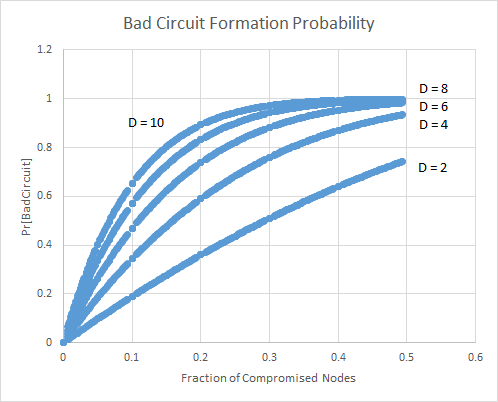
\includegraphics[scale=0.65]{./images/badcircuit.png}
\caption{$\Pr[\mathsf{BadCircuit}]$ behavior as a function of $N$ and $D$ (assuming $W = 1$). As expected, the probability of forming a bad circuit, i.e., one with at least one compromised node, grows logarithmically with the number of compromised nodes in the network.}
\label{fig:badcircuit}
\end{center}
\end{figure}

Figure \ref{fig:badcircuit} illustrates the growth of $\Pr[\mathsf{BadCircuit}]$ as a function of the ratio of compromised nodes for various values for $D$. Observe that this probability quickly grows as $N_{bad} \to N/2$.

For reasonable measures of fault-tolerance, we require that this probability is kept as small as possible. However, for anonymity purposes, we require that $D$ is maximized to achieve optimal mixing cascades (and thus, anonymity) throughout the network. To make this selection in an actual deployment of Boomerang, we would require some apriori knowledge about the expected number of compromised nodes at any given point in time. We are currently not aware of any means of acquiring or estimating this number. Therefore, assuming a reasonable majority of honest nodes, we recommend the selection of $D \in \{4, 5, 6, 7, 8\}$ in order to increase sender anonymity. 

Note that it is possible for the adversary to introduce many invalid addresses into the network. In this case, to keep $\Pr[\mathsf{BadCircuit}]$ small, an honest node can use Boomerang messages to validate addresses so as to aggressively prune invalid addresses from their internal databases. In a similar fashion, Boomerang messages will prune nodes that improperly modify data that is routed through them. Due to the open nature of the Boomerang network, no solution to denial-of-service attacks are currently possible.

% \subsection{Further Security Analysis}
% Analysis assumes a client's first connection is to an honest node. If the client first connects to a malicious node, no security is possible as the malicious node will trivially keep the client in the malicious network. The adversary can use many long-lived identities to bias the distribution of nodes towards the malicious network. If the adversary controls a majority of nodes, no security guarantees are possible.  Therefore, security analysis will assume a client node to be connected to some honest nodes and the adversary does not control the majority of nodes.



